\documentclass[12pt,letterpaper]{article}
\usepackage{anysize}
\usepackage{amsmath}
\marginsize{2cm}{2cm}{1cm}{1cm}
\usepackage{listings}
\usepackage{cite}
\usepackage{caption}
\usepackage{upquote}
\usepackage{xcolor}
\usepackage{xcolor}

\usepackage{graphicx}


\begin{document}

\begin{titlepage}
    \vspace*{4cm}
    \begin{flushleft}
    {\huge
        CS519 Project 3\\[.5cm]
    }
    {\large
        Noisy Displaced Elliptical Dots
    }
    \end{flushleft}
    \vfill
    \rule{5in}{.5mm}\\
    Li Li

\end{titlepage}
\section{source files}
There are only three files lab2.rib, lab2.sl and lab2d.sl.
\section{a simple explanation}
What I did are:
\begin{itemize}
\item Firstly, I looked into third.rib and its respect displacement shader and surface shader. Initially, I did noise to both U and V vector. But later, I just comment out the V vector noise.
\item Basically, my program did similar in both surface shader and displacement shader. In the ecllipse, my surface shader did the displacement calculate and just apply orange to those in the eclipse. However, only in displacement shader I apply the change to the geometry. 
\item For the height, I just do as \bf{float dist = distance( upvp, cntr )*sqrt(Ad*Ad+Bd*Bd);TheHeight = Height-dist*Height;}. These two lines can calculate a certain point(in eclipse) and is distance to the centre of an eclipse. And as the point goes far from the centre it obtain less displacement.
\item For bump-mapping, it just calculate the normals to changed points positions. But the new values of positions are not applied. 
\end{itemize}
\section{result}

\begin{figure}[p]
    \centering
    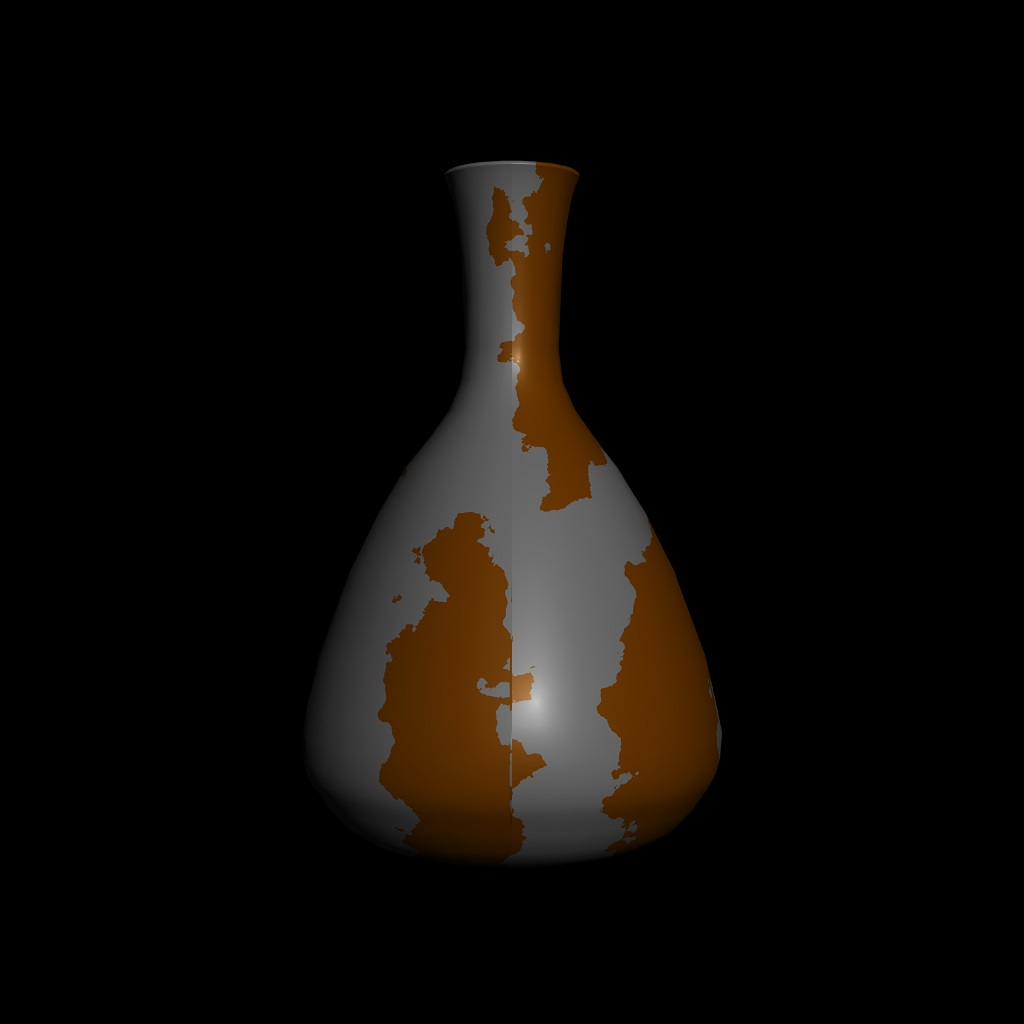
\includegraphics[width=1.\textwidth]{lab2_noise.jpg}
    \caption{1.Surface noise only}
\end{figure}

\begin{figure}[p]
    \centering
    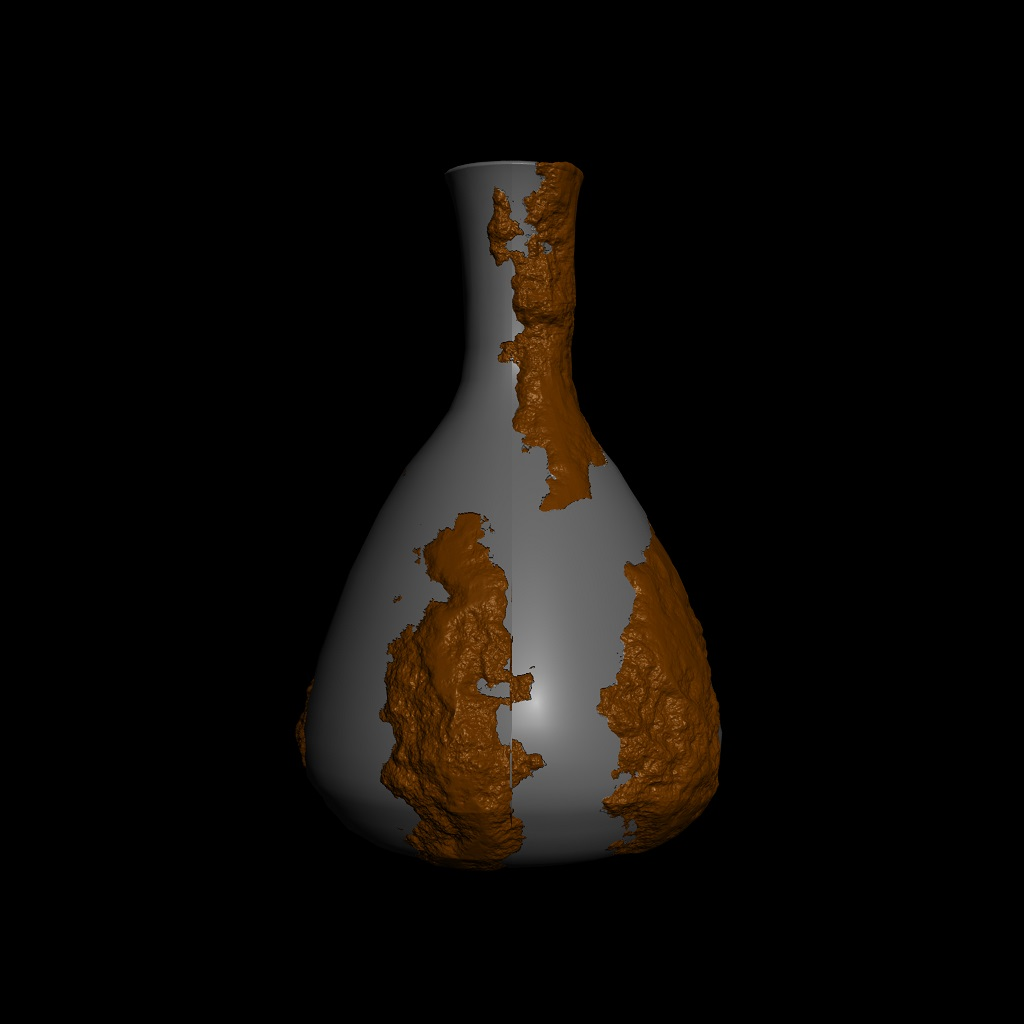
\includegraphics[width=1.\textwidth]{lab2_dis.jpg}
    \caption{2.Surface and Displacement (displacement-mapped) noise}
\end{figure}

\begin{figure}[p]
    \centering
    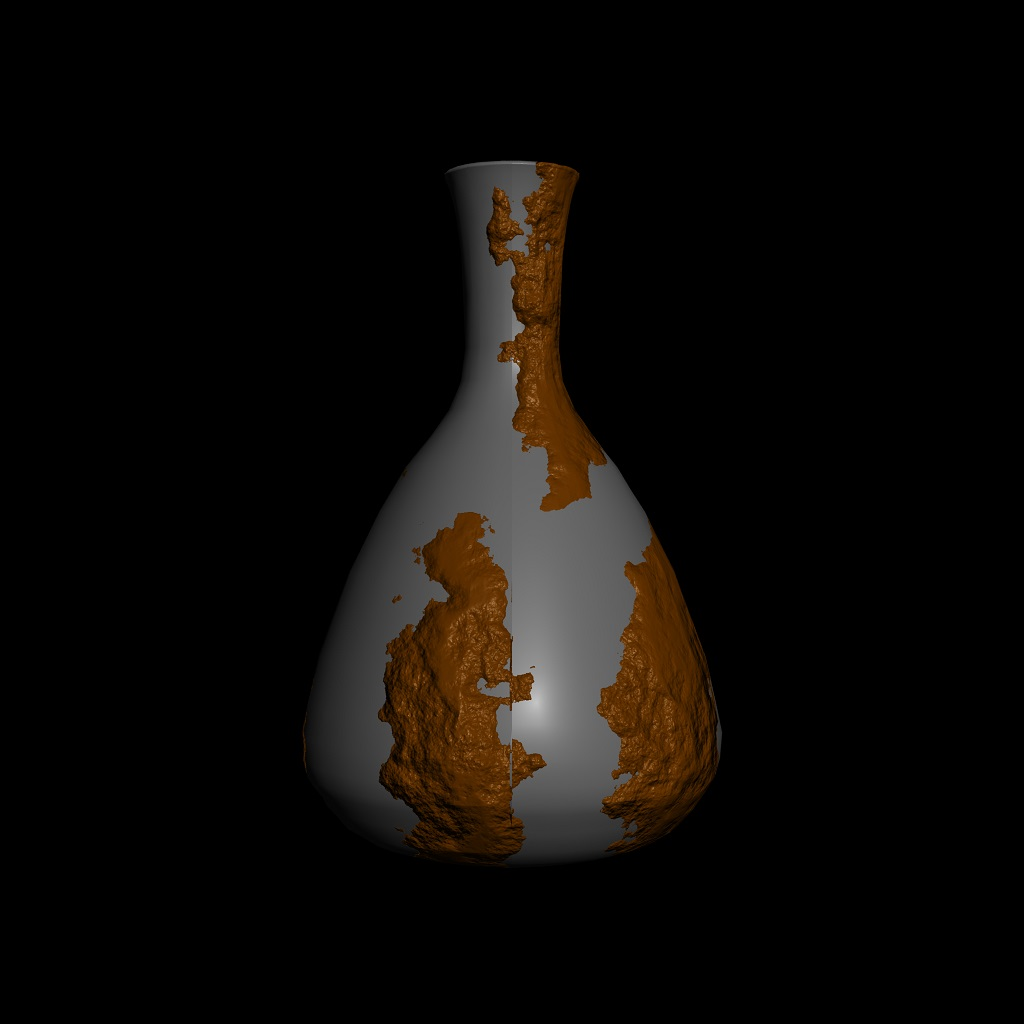
\includegraphics[width=1.\textwidth]{lab2_bump.jpg}
    \caption{3.Surface and Displacement (bump-mapped) noise}
\end{figure}

\end {document}
